\documentclass[border=4pt]{standalone}
\usepackage[T1]{fontenc}
\usepackage{lmodern}
\usepackage{amsmath}
\usepackage{pgfplots}
\pgfplotsset{compat=1.18}
\usepgfplotslibrary{groupplots,fillbetween}
\usetikzlibrary{calc,arrows.meta}
% one colour per kind of method, the same in every figure (Okabe-Ito)
\definecolor{neur}{HTML}{D55E00}   % neurons chosen by attribution
\definecolor{dirc}{HTML}{009E73}   % directions from the weird-vs-normal contrast
\definecolor{read}{HTML}{0072B2}   % readout methods and interventions chosen from readouts
\definecolor{pers}{HTML}{CC79A7}   % Assistant Axis / persona
\definecolor{ctrl}{HTML}{8C8C8C}   % random controls
\definecolor{meas}{HTML}{E69F00}   % measured outcome
\definecolor{ink}{HTML}{222222}
\pgfplotsset{
  every axis/.append style={clip=false, font=\small, axis line style={black!55}, tick style={black!55}, tick align=outside,
    label style={font=\small}, tick label style={font=\footnotesize}, title style={font=\small, align=center}},
  grid style={black!9, line width=0.4pt},
  every axis legend/.append style={font=\footnotesize, draw=none, fill=none},
  ci/.style={/pgfplots/error bars/x dir=both, /pgfplots/error bars/x explicit, /pgfplots/error bars/error bar style={line width=0.8pt}, /pgfplots/error bars/error mark=none},
  yci/.style={/pgfplots/error bars/y dir=both, /pgfplots/error bars/y explicit, /pgfplots/error bars/error bar style={line width=0.8pt}, /pgfplots/error bars/error mark=none},
}

\begin{document}
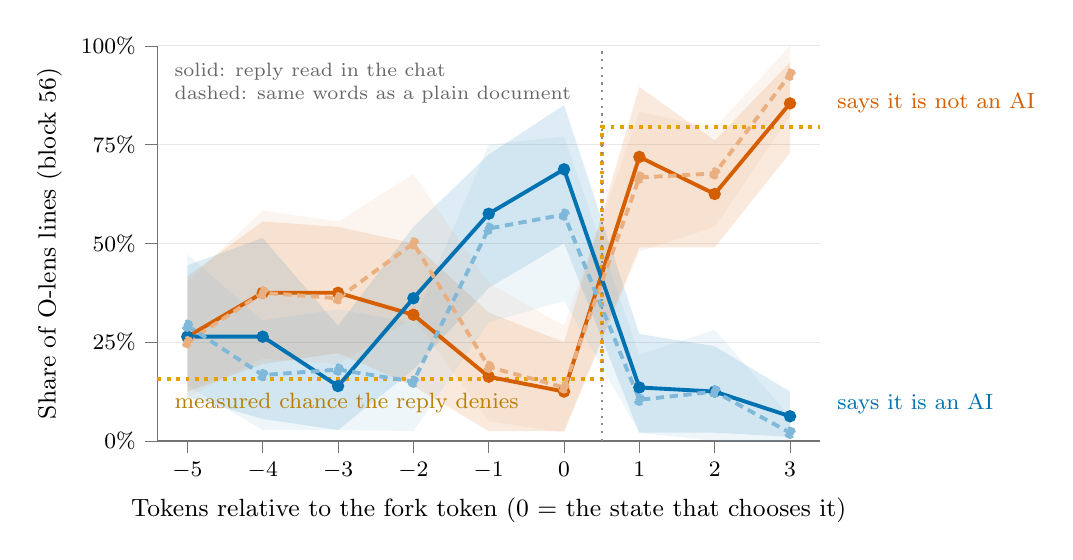
\begin{tikzpicture}
\begin{axis}[width=10cm, height=6.6cm, xmin=-5.4, xmax=3.4, xtick={-5,-4,-3,-2,-1,0,1,2,3}, ymin=0, ymax=100, ytick={0,25,50,75,100}, yticklabel={$\pgfmathprintnumber{\tick}\%$}, axis x line*=bottom, axis y line*=left, ymajorgrids, xlabel={Tokens relative to the fork token (0 = the state that chooses it)}, ylabel={Share of O-lens lines (block 56)}]
\addplot[meas, line width=1.4pt, const plot, dotted] coordinates {(-5.4,15.62) (0.5,15.62) (0.5,79.51) (3.4,79.51)};
\draw[black!45, dotted, line width=0.8pt] (axis cs:0.5,0) -- (axis cs:0.5,100);
\addplot[name path=ua, draw=none] coordinates {(-5,41.67) (-4,55.56) (-3,54.17) (-2,50.03) (-1,32.50) (0,25.00) (1,89.58) (2,76.04) (3,95.83)};\addplot[name path=da, draw=none] coordinates {(-5,12.50) (-4,19.44) (-3,22.22) (-2,13.89) (-1,2.50) (0,2.50) (1,48.96) (2,48.96) (3,72.92)};\addplot[neur, fill opacity=0.13] fill between[of=ua and da];\addplot[neur, line width=1.4pt, mark=*, mark size=1.5pt] coordinates {(-5,26.39) (-4,37.50) (-3,37.50) (-2,31.94) (-1,16.25) (0,12.50) (1,71.88) (2,62.50) (3,85.42)};
\addplot[name path=ub, draw=none] coordinates {(-5,44.44) (-4,51.39) (-3,29.17) (-2,54.17) (-1,72.50) (0,85.00) (1,27.08) (2,23.96) (3,12.50)};\addplot[name path=db, draw=none] coordinates {(-5,11.11) (-4,5.56) (-3,2.78) (-2,18.06) (-1,38.75) (0,50.00) (1,2.08) (2,2.08) (3,1.04)};\addplot[read, fill opacity=0.13] fill between[of=ub and db];\addplot[read, line width=1.4pt, mark=*, mark size=1.5pt] coordinates {(-5,26.39) (-4,26.39) (-3,13.89) (-2,36.11) (-1,57.50) (0,68.75) (1,13.54) (2,12.50) (3,6.25)};
\addplot[name path=uc, draw=none] coordinates {(-5,40.28) (-4,58.33) (-3,55.56) (-2,67.50) (-1,40.00) (0,29.17) (1,83.33) (2,79.17) (3,100.00)};\addplot[name path=dc, draw=none] coordinates {(-5,11.11) (-4,20.83) (-3,19.44) (-2,31.25) (-1,5.00) (0,2.08) (1,47.92) (2,54.17) (3,82.29)};\addplot[neur!50, fill opacity=0.13] fill between[of=uc and dc];\addplot[neur!50, line width=1.4pt, mark=*, mark size=1.5pt, densely dashed] coordinates {(-5,25.00) (-4,37.50) (-3,36.11) (-2,50.00) (-1,18.75) (0,13.54) (1,66.67) (2,67.71) (3,92.71)};
\addplot[name path=ud, draw=none] coordinates {(-5,47.22) (-4,30.56) (-3,33.33) (-2,30.00) (-1,75.00) (0,77.08) (1,21.88) (2,28.12) (3,6.25)};\addplot[name path=dd, draw=none] coordinates {(-5,13.89) (-4,2.78) (-3,2.78) (-2,2.50) (-1,30.00) (0,35.42) (1,2.08) (2,0.00) (3,0.00)};\addplot[read!50, fill opacity=0.13] fill between[of=ud and dd];\addplot[read!50, line width=1.4pt, mark=*, mark size=1.5pt, densely dashed] coordinates {(-5,29.17) (-4,16.67) (-3,18.06) (-2,15.00) (-1,53.75) (0,57.29) (1,10.42) (2,12.50) (3,2.08)};
\node[font=\footnotesize, neur, anchor=west] at (axis cs:3.5,85.42) {says it is not an AI};
\node[font=\footnotesize, read, anchor=west] at (axis cs:3.5,9.25) {says it is an AI};
\node[font=\footnotesize, meas!80!black, anchor=north west] at (axis cs:-5.3,14.62) {measured chance the reply denies};
\node[font=\scriptsize, black!60, anchor=north west, align=left] at (axis cs:-5.3,98) {solid: reply read in the chat\\dashed: same words as a plain document};
\end{axis}
\end{tikzpicture}
\end{document}
